\documentclass[a4paper]{article}
\usepackage{geometry}
 \geometry{
 a4paper,
 total={170mm,257mm},
 left=20mm,
 top=20mm,
 }
\usepackage{multicol}
\usepackage[utf8]{inputenc}
\usepackage[T1]{fontenc}
\usepackage{textcomp}
\usepackage[english]{babel}
\usepackage{amsmath, amssymb}
\usepackage{natbib}
\usepackage{float} 
\usepackage{url}
\usepackage[caption = false]{subfig}
\usepackage{listings}
\lstset{
    breaklines=true,
    basicstyle=\tt\normalsize,
    keywordstyle=\color{blue},
    identifierstyle=\color{magenta},
    frame = single
} 
% figure support
\usepackage{import}
\usepackage{xifthen}
\pdfminorversion=7
\usepackage{pdfpages}
\usepackage{transparent}
\usepackage{subfig}
\usepackage{graphicx}

\pdfsuppresswarningpagegroup=1

\title{\vspace{-2.0cm}Computer Graphics 1MD150 - Project\\ Ray tracing}
\date{}
\author{\vspace{-5cm}Linus Falk}
\begin{document}
\maketitle
\pagenumbering{gobble}

\vspace{-9mm}
\begin{figure}[ht!]
\centering
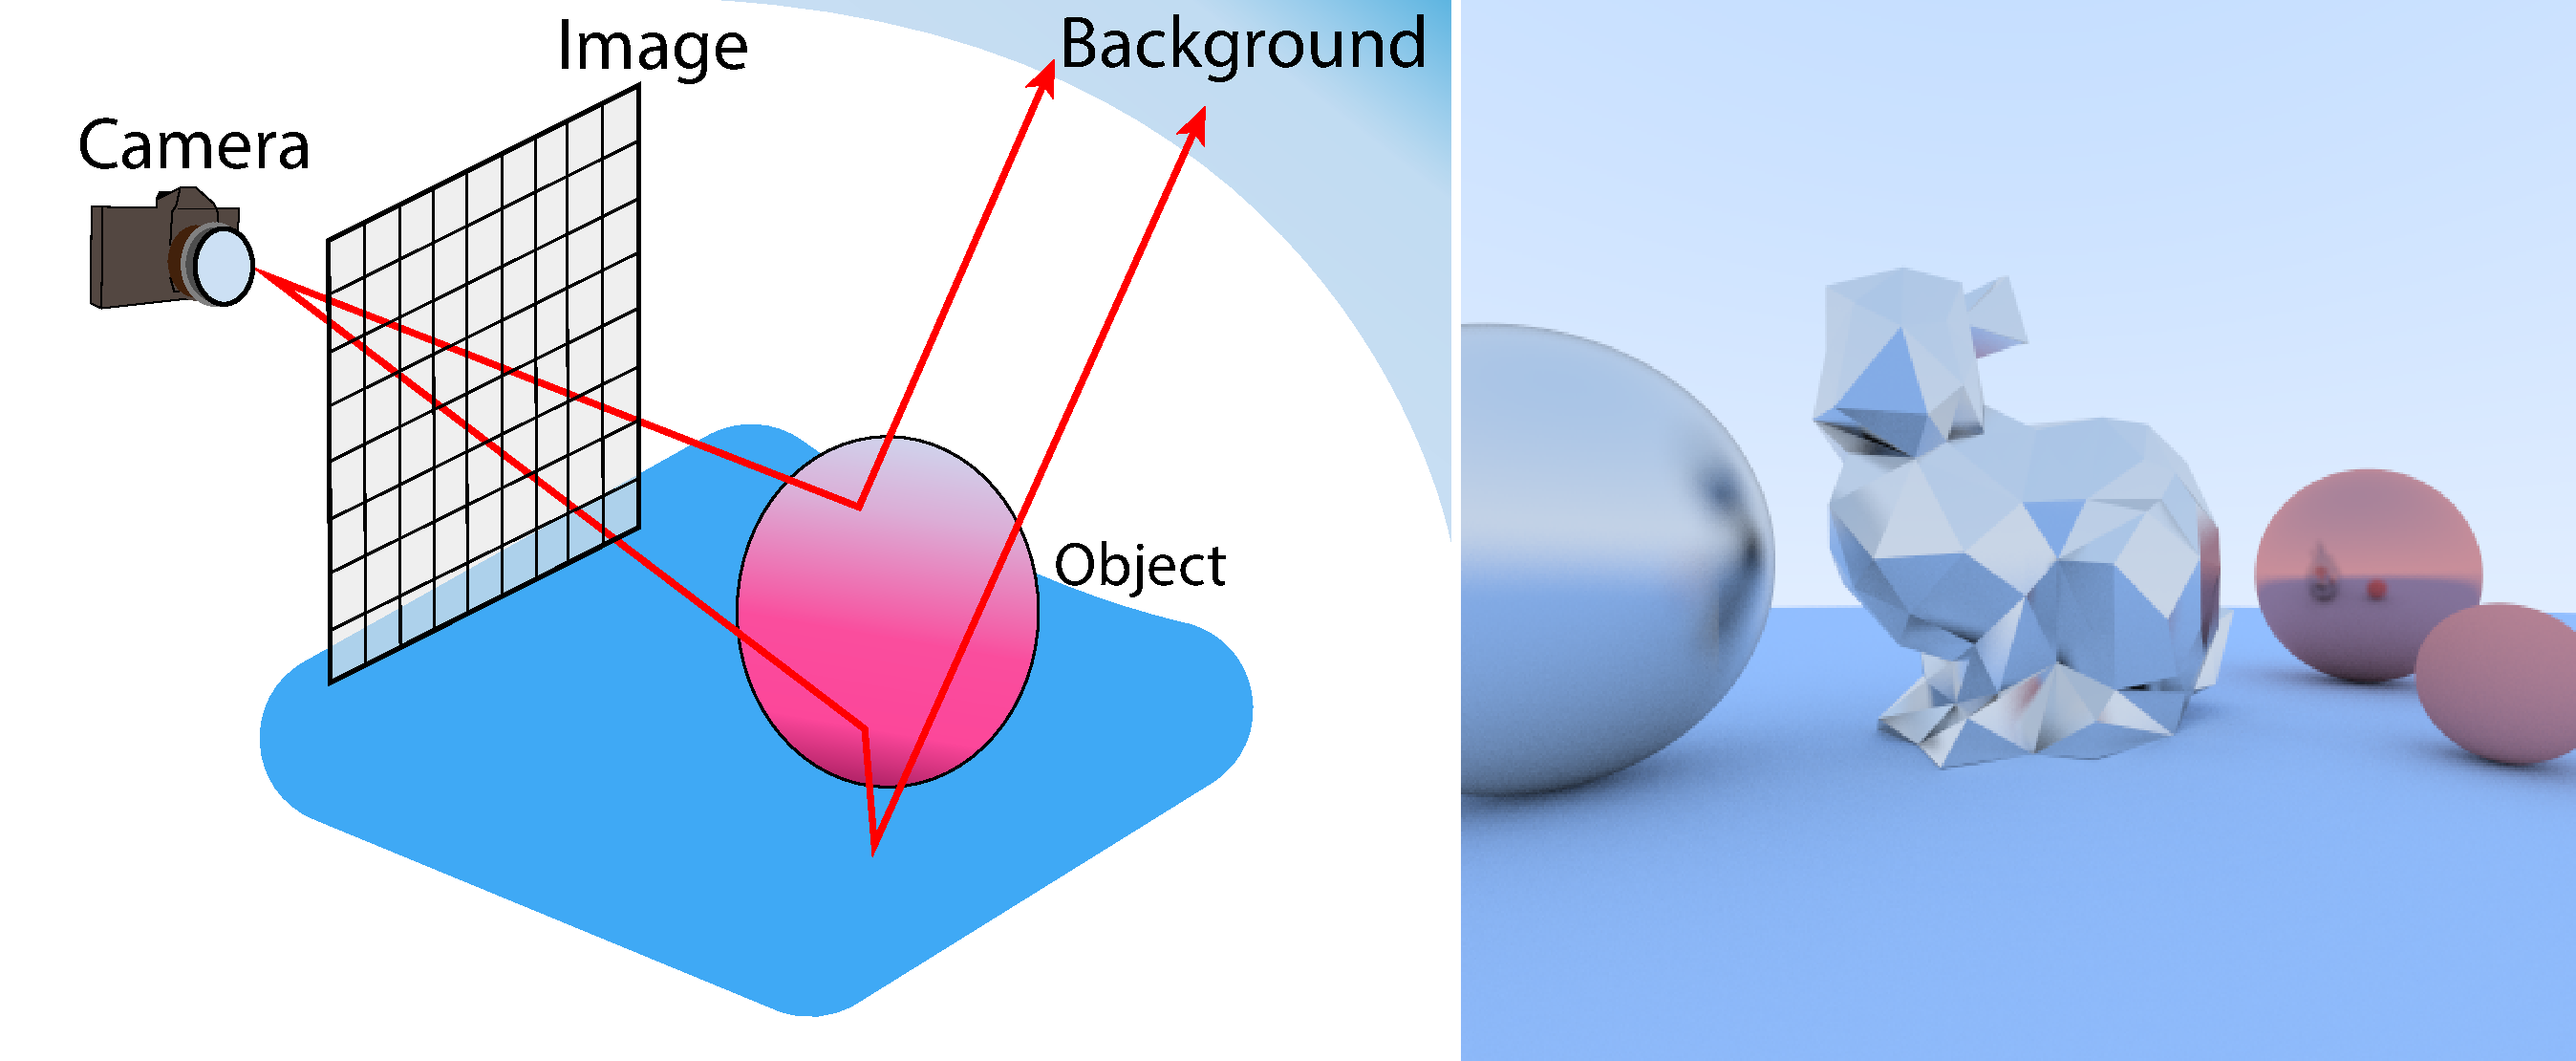
\includegraphics[height=40mm]{figures/cg_project.pdf}
\caption{Concept and result}
\label{fig:example}
\end{figure}



\begin{multicols}{2}
\section*{Ray tracing}\vspace{-2mm}
Ray tracing is a computationally heavy problem to solve, but it offers more realistic lightning (global illumination) for a scene than most other lightning techniques. Although the process is quite straightforward, being recursive, most of the computation lies in calculating the intersections between objects and rays. The recursive stop condition occurs when the the ray no longer intersect any object and only the background color is returned, or when the ray hit the lights source and the color of the light source is returned. The ray intersections with objects can absorb the ray or create a new which pick up the color of the object depending on the objects material properties. By attenuating the color along the ray path from interactions, until it stops by the stopping conditions we get the pixel value of the output pixel \cite{cgbook}.

\vspace{-4mm}\section*{Implementation}\vspace{-2mm}
In this project we implement the ray tracing concept presented above using the CPU for computing the rays and interactions, only utilizing the GPU for rendering the final image. The work was based on the methods in the online book "Ray tracing in one weekend" \cite{Shirley}. The concept above gives an overall good start but to further improve the aesthetics of the result one can start by implementing an \textbf{anti-aliasing filter} to remove the sharp pixelated edges. This was done by averaging multiple samples of each pixels and adding a random intensity to each sample giving us a blurred and more realistic edges. 

\begin{center}
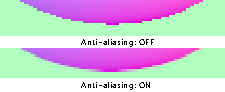
\includegraphics[width= 70mm]{figures/aliasing.pdf}
\end{center}

Material properties control the behavior of the ray when hitting an object. We implemented two types of materials: \textbf{Diffuse} (Lambertian) and \textbf{Metal} (mirror like). When an incoming ray hit the diffuse objects's surface, it takes the incoming ray and randomly scatter it to a new random direction, picking up the color of the object in the process by loosing energy (attenuation). A mirror like metal surface simply reflects the incoming ray according the the incoming angle and the surface of the object. Adding a brushed finish to the metal property was simply done by adding a weighted term of a random direction for the reflected ray. By changing the weight (fuzz) we can control how "brushed" the metal is. For easier demonstration of the material properties was a \textbf{GUI} implemented for changing the parameters color and fuzz. When starting to reflect and redirecting rays with new materials we need to handle the recursive depth of the ray casting process. By setting a GUI controlled variable, we can control the number of bounces and see the effect of computing time. In the introduction, was the computational cost mentioned. One way to reduce this is by incorporating \textbf{bounding volumes} into the solution. Bounding volumes act as a check to see if a ray is going to hit a more complexed-shaped object. If not, it will simply return the background color and we don't need to check which polygon in the object that could be hit. Comparison with the "bunny" object with and without a bounding volume (sphere) yielded a 2 times faster rendering time for the first 5\% of the image with the bounding volume. The final step in order to get a more color accurate image is to implement gamma correction for the display. This was done in the fragment shader with the choice of toggling it on and off in the GUI.  

\vspace{-5mm}
\bibliographystyle{unsrt}
\raggedright
\bibliography{bibliography}

\end{multicols}
\end{document}